\documentclass[sigconf,review,anonymous]{acmart}
\acmConference[ESEC/FSE 2018]{The 26th ACM Joint European Software Engineering Conference and Symposium on the Foundations of Software Engineering}{4--9 November, 2018}{Lake Buena Vista, Florida, United States}
\usepackage{makecell}
\usepackage{todonotes}
\usepackage{graphicx}
\usepackage{color}
\usepackage{tabularx}
\usepackage{subcaption}


\begin{document}

\title{The effect of refactoring test code on production code}
\author{Authors omitted for double-blind review}
\orcid{}
\affiliation{%
  \institution{Institute}
  \streetaddress{Address}
  \city{City} 
  \state{Country} 
  \postcode{}
}
\email{Email}

\newcommand{\ie}{\emph{i.e.},~}
\newcommand{\eg}{\emph{e.g.},~}
\newcommand{\etc}{\emph{etc.}~}
\newcommand{\etal}{\emph{et al.}~}

\begin{abstract}
Refactoring test code is not something developers see in general as an important part of the development process. Despite the fact that this might be true, if the maintainability of the test code gets fully neglected it can have a negative impact on the productivity and throughput of the project. This paper provides an empirical study of test refactors and their impact on the maintainability of the production code. With this research we want to indicate which kind of refactor methods developers apply on their test code, what kind of impact these refactor methods have on the maintainability of the related production code and at last what the correlation is between the maintainability of the test code and the production code.
\end{abstract}
\begin{CCSXML}
<ccs2012>
<concept>
<concept_id>10003120.10003130</concept_id>
<concept_desc>Human-centered computing~Collaborative and social computing</concept_desc>
<concept_significance>500</concept_significance>
</concept>
</ccs2012>
\end{CCSXML}
\ccsdesc[500]{Human-centered computing~Collaborative and social computing}
\keywords{software testing, automated testing, refactoring}
\maketitle

%add more inputs for more files
%\input{content/filename} (omit .tex)
%!TEX root = main.tex

\section{Introduction}
Automated testing is nowadays considered an essential process for 
improving the quality of software systems~\cite{Bertolino2007,Myers2004}, and it is
one of the most common techniques for detecting defects in 
software artifacts~\cite{laitenberger1998studying,van2001refactoring}.
As part of their programming activity, developers write and maintain test code 
continuously~\cite{van2001refactoring}. Zaidman~\etal~\cite{Zaidman2008} investigated the
co-evolution of test and production code, showing that they grow and are modified together.

Several different testing
practices are currently used by practitioners, such as Test Driven Development
\cite{erdogmus2010test}, Mocking~\cite{Spadini}, Extreme Programming \cite{lindstrom2004extreme} or
Acceptance Test-Driven Development \cite{aggarwal2014acceptance}, and many studies on the 
positive effects of testing practices on production code quality have
been carried on in the last decade~\cite{laitenberger1998studying,binder1996testing}. 
Some of these practices,
e.g. Extreme Programming, involve a variety of different refactoring methods.
Van Deursen~\etal~\cite{van2001refactoring} described some refactoring methods 
specifically for test code, such as \textit{Inline Resource}, \textit{Setup External Resource}
or \textit{Reduce Data}. The aim of these refactorings presented by Van Deursen was
to overcome a distinct set of bad smells than involves test code, the so called \textit{test smells}.
However, no studies have studied what type of refactorings developers apply on test
code
Our research deepens the knowledge on these test
refactoring methods by shining light on the impact of refactoring test code on
production code.

One should always take the related production code into consideration when
refactoring the test code. Despite the fact that you might make the code more
readable or maintainable, there is always a chance that the refactor might break
the tests. Of course not every refactor which is made on the test code is to
improve the quality of the project, there are also test code refactors which are
a result of changes which are made in the production code. Nonethless, each
refactor could have an impact on the test code and researching this impact will
allow us to determine the value of test code refactoring.

In order to keep the code readable and maintainable, the size of each of the
classes should be kept to a minimum \cite{baggen2012standardized}. This way it
is easier for the developer to understand what is happening in the code and when
a method or class has to be refactored the impact on the code will be less
significant. Beside the size of a class, the complexity also has an impact on
the maintainability of the test code. Dealing with these problems can increase
the quality of the test code and therefor increase the throughput and
productivity of the development of a project \cite{athanasiou2011constructing}.

Despite the fact that keeping the size and complexity of a class to a minimum
does have a positive effect on the project overall, in practice these methods
are not always complied with. When a project becomes bigger it starts to get
harder to keep it well structured. When the requirements of a project starts to
differ, code changes have to be applied, however these code changes are often
the reason why the maintainability or readability of the project starts to
decrease. This is often because the developers do not realize what kind of
impact refactoring test code can have on the maintainability of a project.

We decided to look at the way developers refactor their test code and if it does
have a positive effect on the related production code. By examining the test
code of multiple projects and evaluating the maintainability we can determine
which of these refactor methods are used and if they do improve the
maintainability of the production code. If the results of this research show
that improving your test code by refactoring bad written code, we might
stimulate developers to do this and improve the overall test code of a project.

During the evaluation of the multiple open-source projects we found out that
during the development of a project, the test code does get refactored a lot.
However, only a small fraction of these refactors was to actually improve the
maintainability of the code. In this paper we will explain how we analyzed these
repositories and which results came out of this evaluation.

% \section{related work}
This work is built upon the research performed by van Deursen et Al. where all kind of test code smells are identified which can be refactored by certain refactor methods \cite{van2001refactoring}. For this research a project was used (DocGen) with a high production/test file ratio. A. van Deursen et Al. classified all the different code refactors to refactor methods which were used to resolve the different test code smells. However, besides the interesting and informative results, this research lacked the overall conviction for developers to do anything more with the presented results. Where van Deursen et Al. focused on Extreme Programming and code smells, we decided to focus more on the default java projects and the maintainability of the project. 

Bois et Al. analyzed the effect of code refactors on the quality of the code \cite{du2004refactoring}. Just like A. van Deursen they searched for all the 'refactoring opportunities' (code smells) and proposed a way to refactor the code to enhance certain properties of the maintainability. They encountered many problems in classifying the analyzed code into refactor methods, however they were able to make certain guidelines for developers which, if followed, should improve the code quality of a project. Just like Bois et Al. we hope to stimulate developers to increase the quality of their project by refactoring the test code with the right refactor methods.

Increasing the quality of the code has been a driving force for analyzing code refactors by many studies. However, 'code quality' is a very broad concept which can't be formulated to one specific value. Subramanyam et Al. \cite{subramanyam2003empirical} did an empirical study on the role of object-oriented design complexity metrics in determining software defects. They used a tool (CK) which was able to analyze all the maintainability metrics of a software project. This study provided a convincing correlation between certain CK metrics and software defects.

Another approach for improving the code quality is by testing it extensively. Laitenberger et Al. \cite{laitenberger1998studying} studied the effects of code inspection and structural testing on the quality of the software. He concluded besides the importance of code inspection, that testing code is a very important requirement for detecting bugs and thereby improving the code quality.
%!TEX root = ./main.tex

\section{Methodology}
In this paper we aim to understand what type of refactorings developers apply the most on test code, as well as identifying the effects of those refactorings on production code. To this aim, we analyzed 3 open-source projects using a variety of available tools. In this section we elaborate on the chosen data-sources, research tools and the research questions we attempt to answer.

\subsection{Research Questions}
\label{rqs}
Below we will describe the research questions we will be answering in this paper.\\
\indent\textbf{RQ1} \textit{What type of refactorings do developers apply on test code?}\\
We want to identify what kind of refactoring methods developers apply to test code and see if we find any relation to the methods described in \cite{van2001refactoring}. We also want to look into the possible correlations to refactor methods applied to different types of system components.\\
\indent\textbf{RQ2} \textit{What is the relation between test code maintainability and production code maintainability?}\\
We aim to see whether there is a relation between test code maintainability and production code maintainability, so if an improvement or deterioration in test code maintainability also affects the production code. 

\subsection{Projects under investigation}
As subject systems for our study we consider 3 OSS projects and their 667 releases. The selection is driven by two main factors: firstly, since we have to run static analysis tools to different test refactorings and compute maintainability metrics, we focus on projects whose source code is publicly available (i.e., OSS); secondly, we analyze systems having a big corpus of test code. After filtering on these criteria, we randomly select 3 OSS projects from the list available on GitHub~\footnote{\url{https://github.com}} having different size, a big amount of releases and with a number of JUnit test cases higher than 1,000 in all the releases.

The used projects can be found in Table~\ref{table:1}. The repositories exists out of multiple projects which are either maven or gradle projects, containing a production and a test code directory. This project setup makes it more easier to find production/test pair files, which is very important for this research. All projects have a time span of at least 5 years and have over 150 releases, which means that there is a strong possibility that multiple refactors have been done in order to maintain the code.


\begin{table}[htb]
    \caption{An overview of the analysed projects}
    \label{table:1}
    \resizebox{0.8\columnwidth}{!}{%
    \begin{tabular}{lrrr} 
     \hline 
     \textbf{Project name} & \thead{\# of prod.\\files} & \thead{\# of test\\files} & \thead{\# of\\releases} \\
     \hline
     SonarQube & 3166 & 2085 & 165 \\
     Apache Hadoop & 5880 & 2498 & 288 \\ 
     ElasticSearch & 3667 & 1328 & 214 \\
     \hline
    \end{tabular}
    }
\end{table}

\subsection{Defining Maintainability}
\label{sec:maint-metric}
Since the notion of maintainability is not defined in literature, in this work we take into consideration previous studies' definitions and we create our own version of maintainability. 
On first sight one might be tempted to use the maintainability index~\footnote{\url{https://blogs.msdn.microsoft.com/zainnab/2011/05/26/code-metrics-maintainability-index/}}, however, previous studies~\cite{sjoberg2012questioning, heitlager2007practical} have demonstrated that the metric has some unreliable properties. The maintainability index can be a tool to help a developer improve his/her code, but can not be used to conclude if a project/class has a high maintainability or not. 

Research has showed \cite{sjoberg2012questioning} that the most reliable metrics of maintainability are the size of the project and the inverse cohesion. Metrics as \textbf{LOC} (Lines of Code), \textbf{NOF} (Number of Fields) and \textbf{NOM} (Number of Methods) all give some indication about the size of a class and are thereby more reliable for determining the maintainability. As in previous studies~\cite{citationneeded}, to create our version of maintainability index we also take into consideration the complexity of a class (\textbf{WMC}).

At the end, our own maintainability analysis method is based on the LOC, NOF, WMC and NOM of a Java file. Each metric is divided into 4 categories: ``Very Low'', ``Low'', ``Medium'' and ``High'', representing the risk of being poorly maintainable. As done in previous studies~\cite{alves2010deriving}, we base the boundaries of these categories on our own dataset, by taking the 70th, 80th and 90th quantile.

% \begin{table}[!ht]
%     \centering
%     \label{categories-LOC}
%     \begin{tabular}{|l|l|}
%         \hline
%         \textbf{Condition} & \textbf{Category} \\
%         \hline
%         x < 126 & Very Low \\
%         126 < x < 173 & Low \\
%         173 < x < 281 & Medium \\
%         281 < x & High \\
%         \hline
%     \end{tabular}
%     \caption{LOC maintainability categories}
% \end{table}
% \begin{table}[!ht]
%     \centering
%     \label{categories-NOF}
%     \begin{tabular}{|l|l|}
%         \hline
%         \textbf{Condition} & \textbf{Category} \\
%         \hline
%         x < 3 & Very Low \\
%         3 < x < 5 & Low \\
%         5 < x < 9 & Medium \\
%         9 < x & High \\
%         \hline
%     \end{tabular}
%     \caption{NOF maintainability categories}
% \end{table}
% \begin{table}[!ht]
%     \centering
%     \label{categories-WMC}
%     \begin{tabular}{|l|l|}
%         \hline
%         \textbf{Condition} & \textbf{Category} \\
%         \hline
%         x < 17 & Very Low \\
%         17 < x < 26 & Low \\
%         26 < x < 46 & Medium \\
%         46 < x & High \\
%         \hline
%     \end{tabular}
%     \caption{WMC maintainability categories}
% \end{table}
% \begin{table}[!ht]
%     \centering
%     \label{categories-NOM}
%     \begin{tabular}{|l|l|}
%         \hline
%         \textbf{Condition} & \textbf{Category} \\
%         \hline
%         x < 9 & Very Low \\
%         9 < x < 13 & Low \\
%         13 < x < 20 & Medium \\
%         20 < x & High \\
%         \hline
%     \end{tabular}
%     \caption{NOM maintainability categories}
% \end{table}

\subsection{Data Extraction}
\label{data-extraction}
To answer our research questions, we extracted information regarding the maintainability of a project and the types of refactorings developers apply the most on test code. To this aim, we use 3 OSS tools (they all can be found on GitHub): 
\begin{itemize}
    \item \textbf{Repodriller}: Java framework that allows the extraction of information such as commits, modifications, diffs, and source code. We used it to mine the change history information of the subject systems
    \item \textbf{CK}: Java tool to extract code metrics of Java systems
    \item \textbf{Refactoring-miner}: library written in Java that can detect refactorings applied in the history of a Java project.
\end{itemize}

To answer RQ$_1$, namely what type of refactorings developers apply the most on test code, we run the tool Refactoring-miner on all the commits of the subject systems on the last 5 years. We decided to narrow the total amount of considered commits since this process is highly time consuming. 
% To answer RQ$_2$, we collect information regarding the impact of test code refactoring on production code. For every commit of the last 5 years, we first check if there are actually any refactors made on test code: If this is not the case we skip the whole commit because it does not contain relevant information for this research question. Instead, if the commit does contain refactors, for every refactored test file we fetch the matching production class and calculate the metrics of this file every 10 commits for 5 versions (\ie we calculate the metrics of the file after 10, 20, 30, 40, 50 commits) after the test refactoring had taken place. To match the production class we exploit a traceability technique based on naming convention, \ie, it identifies the methods under test by removing the string ‘Test’ from the method name of the JUnit test method. This technique has been previously evaluated by Sneed~\cite{sneed2004reverse}, demonstrating the highest performance (both in terms of accuracy and scalability) with respect to other traceability approaches (e.g., slicing-based approaches~\cite{qusef2014recovering}). 
To answer RQ$_2$ and study the relation between test and production code maintainability, we collect monthly metrics of the systems and then map every production file to its test file. To correctly match the two types of files, we exploit a traceability technique based on naming convention, \ie, it identifies the methods under test by removing the string ‘Test’ from the method name of the JUnit test method. This technique has been previously evaluated by Sneed~\cite{sneed2004reverse}, demonstrating the highest performance (both in terms of accuracy and scalability) with respect to other traceability approaches (e.g., slicing-based approaches~\cite{qusef2014recovering}). 
For this research question, we decided to consider all the history of the projects (instead of only 5 years as previously done for RQ$_1$), but on a monthly base. More specifically, for all the subject systems, we monthly checkout the code base and collect the metrics of the entire system using \emph{CK}. 

The details about the data extraction can be found in Table.~\ref{table:6}.

\begin{table}[htb]
\caption{Statistics of the 3 projects.}
\label{table:6}
\resizebox{\columnwidth}{!}{%
\begin{tabular}{lrrr}
 & Sonarqube & Hadoop & Elasticsearch \\
\hline
\begin{tabular}[c]{@{}l@{}}Amount of monthly\\metrics commits\end{tabular} & 55 & 77 & 45 \\ 
\hline
\begin{tabular}[c]{@{}l@{}}Average amount of\\evaluated Java files\end{tabular} & 3170 & 1466 & 3875 \\ 
\hline
\begin{tabular}[c]{@{}l@{}}Total amount of\\test refactors\end{tabular} & 6832 & 5452 & 10933\\
\hline
\end{tabular}
}
\end{table}

% \section{Implementation}
In this section we want to give a high level explanation of our implementation for mining and processing the data we use to tend to our research questions. We first discuss the mining process and secondly the processing of the mined data.
\subsection{Mining the data}
In order to answer the three research questions we need information about the maintainability of a project, all the refactors which are made and the correlation between these two datasets. To collect this information the tool \textit{Repodriller} was used to iterate through all the commits of a repository and checkout each commit in order to process each file in the current state of the repository when the commit was made. However, we were not able to mine all the information at once, so we decided to make 2 different data-mining jobs: the \textbf{monthly metrics job} and the \textbf{refactoring job}. For both of these jobs we have decided to mine only the last 5 years of each project's history. We made this choice to reduce the amount of time the jobs would take to run and this way we still have a significant part of the project's history.

The monthly metrics job is the first data-mining job which collects all the information about the maintainability and the production-test pairs from the commits of a project on a monthly basis. We calculate all the metrics with the \textit{CK} tool which are described in section \ref{Researchtools}. 
%When all these metrics are calculated, we count all the operators and operands in order to calculate the \textit{Hallstead Volume}. We use the \textit{Hallstead Volume} together with the \textit{LOC} and the \textit{WMC} to calculate the \textit{Maintainability Index}. 

From this point on we have all the metrics which are relevant to the maintainability of the file, which we can use for the \textit{Monthly Metrics} file. In order to find the correlation between the production and test code, we have to find the production-test pairs. Because all the repositories exists out of either gradle or maven projects, we can find the relevant test file of each production file by naming conventions and by using the project structure. JUnit test classes are often named after their respective production classname + Test, so for example a production class "FileCacheProvider" would have a test class called "FileCacheProviderTest". Java projects often have a structure with a "main" and "test" source folder, each having a similar substructure, making finding test classes easier. The found pairs we write to the \textit{class-pair file}.

The refactoring job is the second data-mining job which collects all the information about the refactors of test classes and tracks matching production classes of test classes. First we check if there are actually any refactors made in the commit. If this is not the case we can skip the whole commit because it contains no relevant information for this research. However, if the commit does contain refactors we collect all the refactor methods which were used on the test code and write this information to the \textit{test refactor file}. We then fetch the matching production class from the \textit{class-pair file} and calculate the metrics of this file every 10 commits for 5 versions, 10-20-30 etc commits after the test refactoring had taken place. We write the metrics of the tracked production files to the \textit{impact production file} with the commithash of the commit in which the test refactoring happened as an identifier. When this information is collected we tend to the correlation between refactors on test code and the maintainability of the production code. 

\subsection{Processing the data}
For processing the collected data we have used several methods, for research question 1 it was sufficient to use Microsoft Excel for counting the different types of refactorings found in the \textit{test refactors file}.

For research question 2 and 3 we have written a Java implementation that loads the relevant files and the plots that will be seen later in this work were made using JFreeChart \footnote{http://www.jfree.org/jfreechart/}. We would like to point the reader to the public git repository where the code as well as the found data is hosted \footnote{https://github.com/Dahny/Software\_Analytics}.
%!TEX root = ./main.tex
\section{Results}
This section describes the results to our research questions aimed at understanding the types of refactoring developers apply the most on test code as well as their impact on production code maintainability. 

\noindent
\subsection*{RQ1: What type of refactorings do developers apply on test code?}
To find what types of refactorings developers apply the most on test code, we used Refactor-miner on our subject systems. The results can be found in Table~\ref{table:9}.
% \ifx true false

% \begin{table}[!ht]
% \centering
% \begin{tabular}{|l|l|l|l|}
% \hline
% \multicolumn{4}{|c|}{Sonarqube} \\ \hline
% Extract Method & 315 & Pull Up Attribute & 33 \\ \hline
% Move Class & 1118 & Extract Superclass & 12 \\ \hline
% Move Attribute & 341 & Push Down Method & 37 \\ \hline
% Rename Package & 6 &  Push Down Attribute & 3 \\ \hline
% Move Method & 553 & Extract Interface & 1 \\ \hline
% Inline Method & 53 & Rename Class & 820 \\ \hline
% Pull Up Method & 59 & Rename Method & 3481 \\ \hline
% \end{tabular}
% \caption{Amount of refactorings by type in sonarqube}
% \label{table:9}
% \end{table}

% \begin{table}[!ht]
% \centering
% \begin{tabular}{|l|l|l|l|}
% \hline
% \multicolumn{4}{|c|}{Hadoop} \\ \hline
% Extract Method & 1690 & Pull Up Attribute & 152 \\ \hline
% Move Class & 261 & Extract Superclass & 46 \\ \hline
% Move Attribute & 395 & Push Down Method & 2 \\ \hline
% Rename Package & 0 &  Push Down Attribute & 0 \\ \hline
% Move Method & 721 & Extract Interface & 3 \\ \hline
% Inline Method & 89 & Rename Class & 555 \\ \hline
% Pull Up Method & 175 & Rename Method & 1363 \\ \hline
% \end{tabular}
% \caption{Amount of refactorings by type in hadoop}
% \label{table:10}
% \end{table}

% \begin{table}[!ht]
% \centering
% \begin{tabular}{|l|l|l|l|}
% \hline
% \multicolumn{4}{|c|}{Elasticsearch} \\ \hline
% Extract Method & 565 & Pull Up Attribute & 23 \\ \hline
% Move Class & 1363 & Extract Superclass & 73 \\ \hline
% Move Attribute & 282 & Push Down Method & 298 \\ \hline
% Rename Package & 6 &  Push Down Attribute & 100 \\ \hline
% Move Method & 1071 & Extract Interface & 0 \\ \hline
% Inline Method & 57 & Rename Class & 2401 \\ \hline
% Pull Up Method & 311 & Rename Method & 4370 \\ \hline
% \end{tabular}
% \caption{Amount of refactorings by type in elasticsearch}
% \label{table:11}
% \end{table}

% \fi

\begin{table}[!ht]
\caption{Refactorings by type in the subject systems.}
\label{table:9}
\resizebox{\columnwidth}{!}{%
\begin{tabular}{lrrrrrr}
\hline
 & Sonarqube & Hadoop & Elasticsearch & Total \\ \hline
Rename Method & 3481 & 1363 & 4370 & 9214 \\
Move Class & 1118 & 261 & 1363 & 2742 \\
Rename Class & 820 & 555 & 2401 & 3776 \\
Move Method & 553 & 721 & 1071 & 2345 \\
Move Attribute & 341 & 395 & 282 & 1018 \\
Extract Method & 315 & 1690 & 565 & 2570 \\
Pull Up Attribute & 33 & 152 & 23 & 208 \\
Extract Superclass & 12 & 46 & 73 & 131 \\
Push Down Method & 37 & 2 & 298 & 337 \\
Rename Package & 6 & 0 & 6 & 12 \\
Push Down Attribute & 3 & 0 & 100 & 103 \\
Extract Interface & 1 & 3 & 0 & 4 \\
Inline Method & 53 & 89 & 57 & 199 \\
Pull Up Method & 59 & 175 & 311 & 545 \\
\end{tabular}
}
\end{table}

\begin{figure}[!ht]
 \centering
 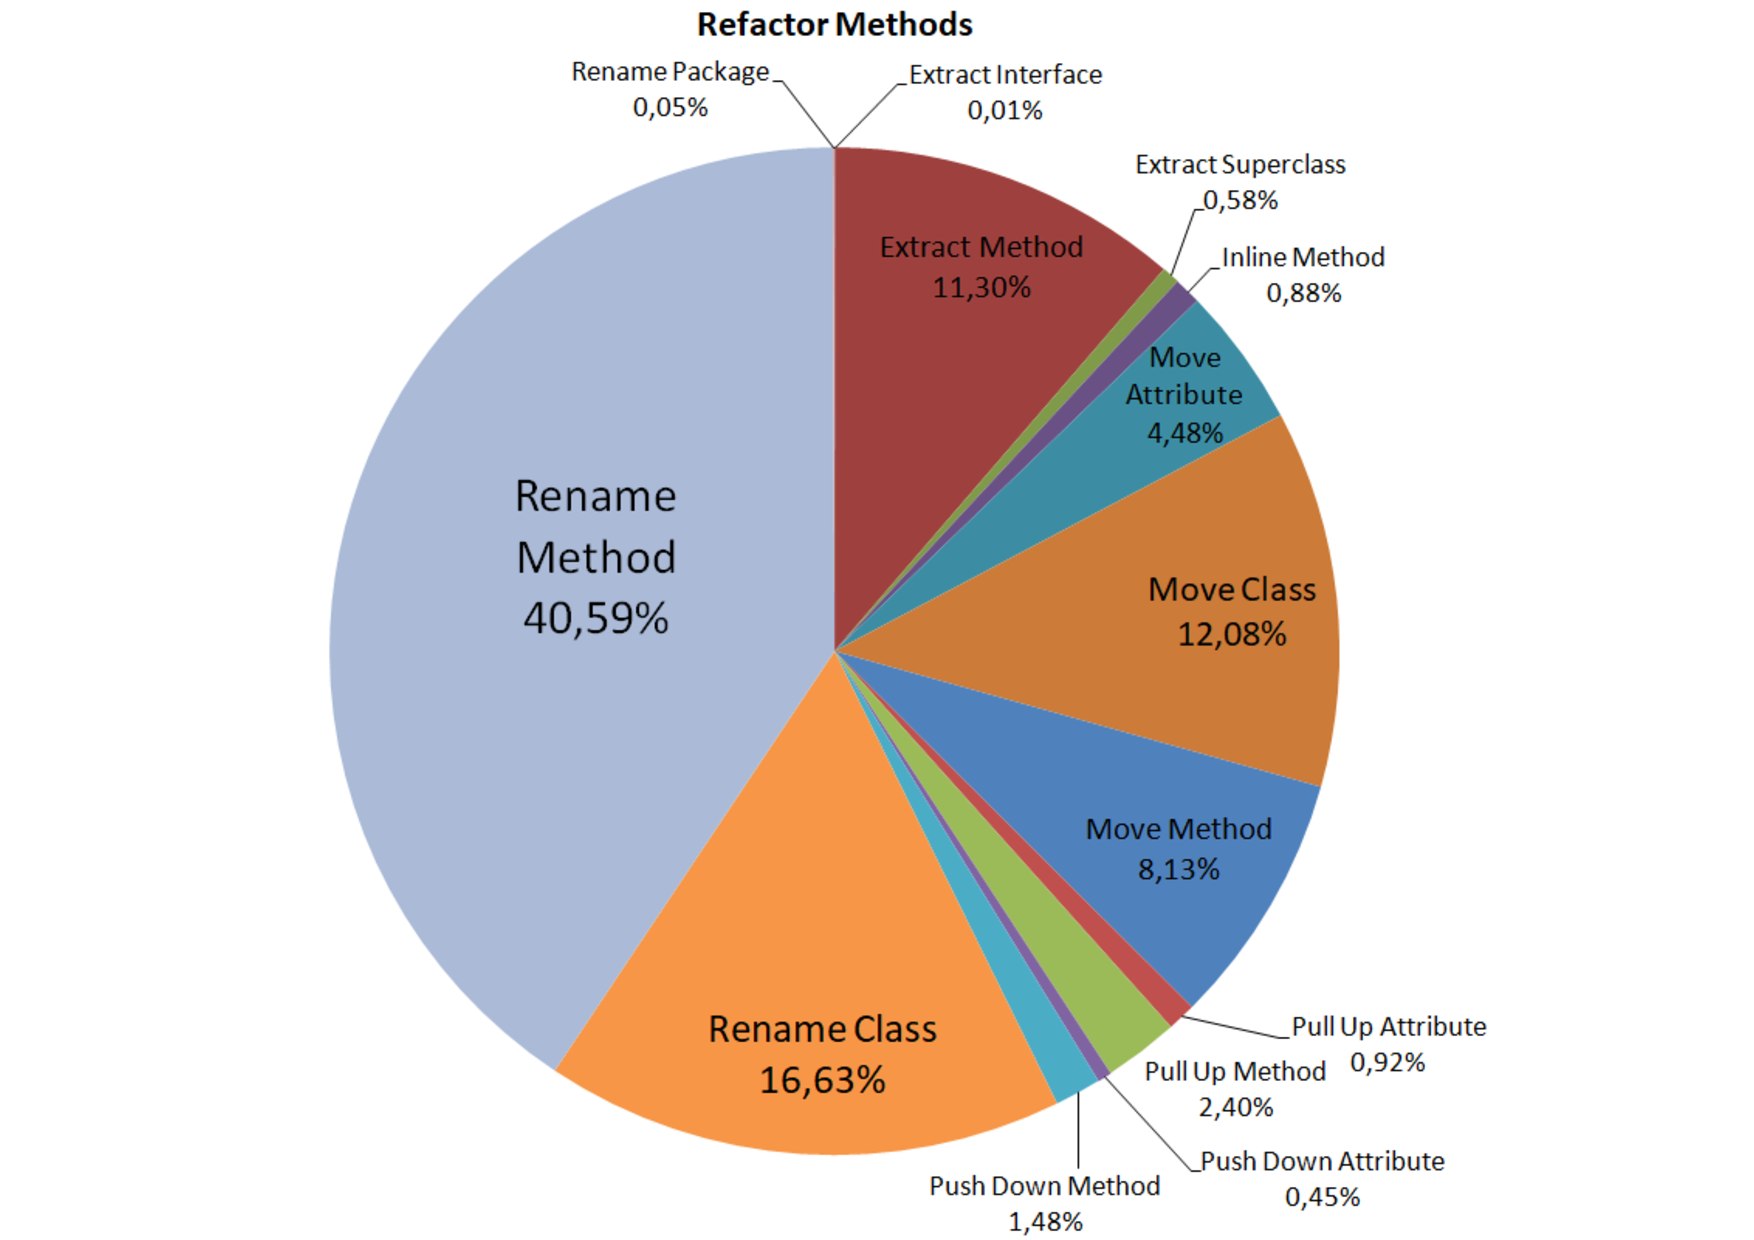
\includegraphics[width=\columnwidth]{resources/refactorMethods.pdf}
 \caption{Percentages of the refactor methods of all the repositories}
 \label{figure:piechart}
\end{figure}

As we can notice, some refactor methods were used more often than others. The most popular refactor method for test code would be \textit{Rename Method}. The refactor methods \textit{Rename Class}, \textit{Move Class} and \textit{Extract Method} were also used often. These methods are used for improving the names and location of codes, but also for giving the code a more logical structure. Refactor methods like \textit{Rename Package}, \textit{Extract Interface}, \textit{Extract Superclass}, \textit{Push Down Method} and \textit{Push Down Attribute} were instead barely used. Another result we can notice is that some of the refactor methods were used much more in a project than in the others. For instance, \textit{Extract Method} was used much more in the Hadoop than in Sonarqube or Elasticsearch. We speculate that this might happen because each project has their own "rules of code quality" that developers have to apply, as well as their own ideas about refactoring code (for example, some projects can have more strict rules and force developers to refactor test code).

Given our experimental setting, we cannot speculate on the motivations behind the results achieved so far: indeed, our RQ$_1$ meant to be a coarse-grained investigation aimed at understanding what types of refactorings developers apply the most. Thus, in this research question we did not focus on the reasons behind these refactorings, \eg are the test refactored due to a change in the production code? or maybe because developers were close to a new release? Our RQ$_3$ makes a first step in providing additional insights on such a relationship, however further research should better investigate this relationship.

%In the \textit{Sonarqube} project, the refactor method \textit{Rename Method} seems to be used far more often than in the \textit{Hadoop} project. The same can be said about the refactor method \textit{Extract Method}, which is used far more often in the Hadoop project as in the Sonarqube project. Ofcourse, each project has its own difficulties and thereby their own refactorings. 

%-----------------------------------------------------------------------------------------------
% \subsection*{RQ2: Does the refactoring of test code affect the maintainability of production code?}\label{maintainability:improved}
% In this section we want to adres the results found that have been collected in an attempt to answer RQ2. Refactor data on test classes has been gathered and their matching production classes were checked every 10 commits after that for 5 versions in total, so up to 50 commits ahead. As mentioned in the explanation of RQ2 we will be looking at refactors on test code that significantly improved the maintainability of that test class. We define a significant improvement as a summed difference in the classes each metric among LOC, NOF, NOM and WMC. An example, a class that went from Medium to Low in terms of LOC, has a difference of 1 in terms of LOC. High to Very Low is a difference of 4, Low to High is a difference of -2. Adding the difference for each metric gives us the summed difference, if this value exceeds 4 we say the improvement is significant.  Among all projects we have found the follwing numbers:
% \begin{table}[!ht]
%     \centering
%     \begin{tabular}{|l|l|}
%         \hline
%         \multicolumn{2}{|c|}{Test refactorings} \\ \hline
%         Total & 1756 \\ \hline
%         Worsened & 236 \\ \hline
%         Unaffected & 824 \\ \hline
%         Improved & 696 \\ \hline
%         Significantly improved & 108 \\ \hline
%     \end{tabular}
%     \caption{Counts of test refactorings and how they affected maintainability}
%     \label{table:12}
% \end{table}
% We then check the first and last version of the matching production class that was tracked and calculate the difference here as well. Some production files could not be tracked, this can be accounted to rename or deletions of the file causing our code to be unable to find the file.
% \begin{table}[!ht]
%     \centering
%     \begin{tabular}{|l|l|}
%         \hline
%         \multicolumn{2}{|c|}{Tracked production files} \\ \hline
%         Total & 108 \\ \hline
%         Affected & 0 \\ \hline
%         Unaffected & 85 \\ \hline
%         Error in tracking & 23 \\ \hline
%     \end{tabular}
%     \caption{Tracked production files' maintainability after significant maintainability improving test refactor}
%     \label{table:13}
% \end{table}
% Surprising not a single production file was modified significantly (i.e. causing a shift in its classification among the metrics we look at). Suggesting that it is very unlikely that a refactoring in test code that significantly improves maintainability causes a similar improvement in the production class under test. Now this result is not what we were expecting, now this is also something that might be related to the projects under analysis, updating test code might not happen before updating the production class, perhaps it is the other way around, production code first, after which test code gets updated. Perhaps it happens more in a periods of pure testing and pure development, such period have also been identified by \cite{zaidman2008mining}. This way our method by looking up to 50 commits in the future after a test code refactoring, does not find the corresponding production file change, if present at all. On the other hand if testing and development are done in different periods then we cannot accredit a test code refactoring to cause a change in production code.

%-----------------------------------------------------------------------------------------------
\subsection*{RQ2: What is the correlation between test code maintainability and production code maintainability?}
\label{maintainability:correlation}
Using the categories defined in Section~\ref{sec:maint-metric}, we have categorized the risk for each pair Production-Test class for all the metrics. As shown in Table~\ref{table:6}, we mined a total of 177 snapshots: Since plotting all the snapshots would result in too much data, we have chosen to visualise only 5 snapshots (randomly selected) for each project, hence 15 in total. 

In Figure~\ref{fig:heat_map} we show the result. On the axis we can find the risk categories: The X-axis shows the category in which the test class is classified, while the Y-axis shows the category of the corresponding production class. 

\subsubsection{Analyzing the results}
Throughout all the metrics we have analyzed in every project we see a strong correlation in production and test classes both being classified in the Very Low risk category. This correlation is not that present in the other categories, and this holds for each metric. We do however notice a high density in the leftmost column in each plot: This indicates that where production classes are being classified in a variety of categories, the vast majority of test classes is classified in the Very Low risk category. This can be attributed to the general lower complexity of a test class compared to a production class. For example, a highly complex production class can still be tested with a relatively simple test class that verifies if the output of certain functions is as expected.

The high density in the Very Low category for both test and production classes is a surprising result: for each of these metrics it holds that where a production class is categorized as low risk, so is the corresponding test class, giving an indication that a relation is present. However we do not see this density in the "Low/Low", "Medium/Medium" and "High/High" categories: As previously discussed, this can be led back to the argument presented earlier, that even higher complexity classes can be tested using relatively simple test classes.

\begin{figure*}
    \centering
    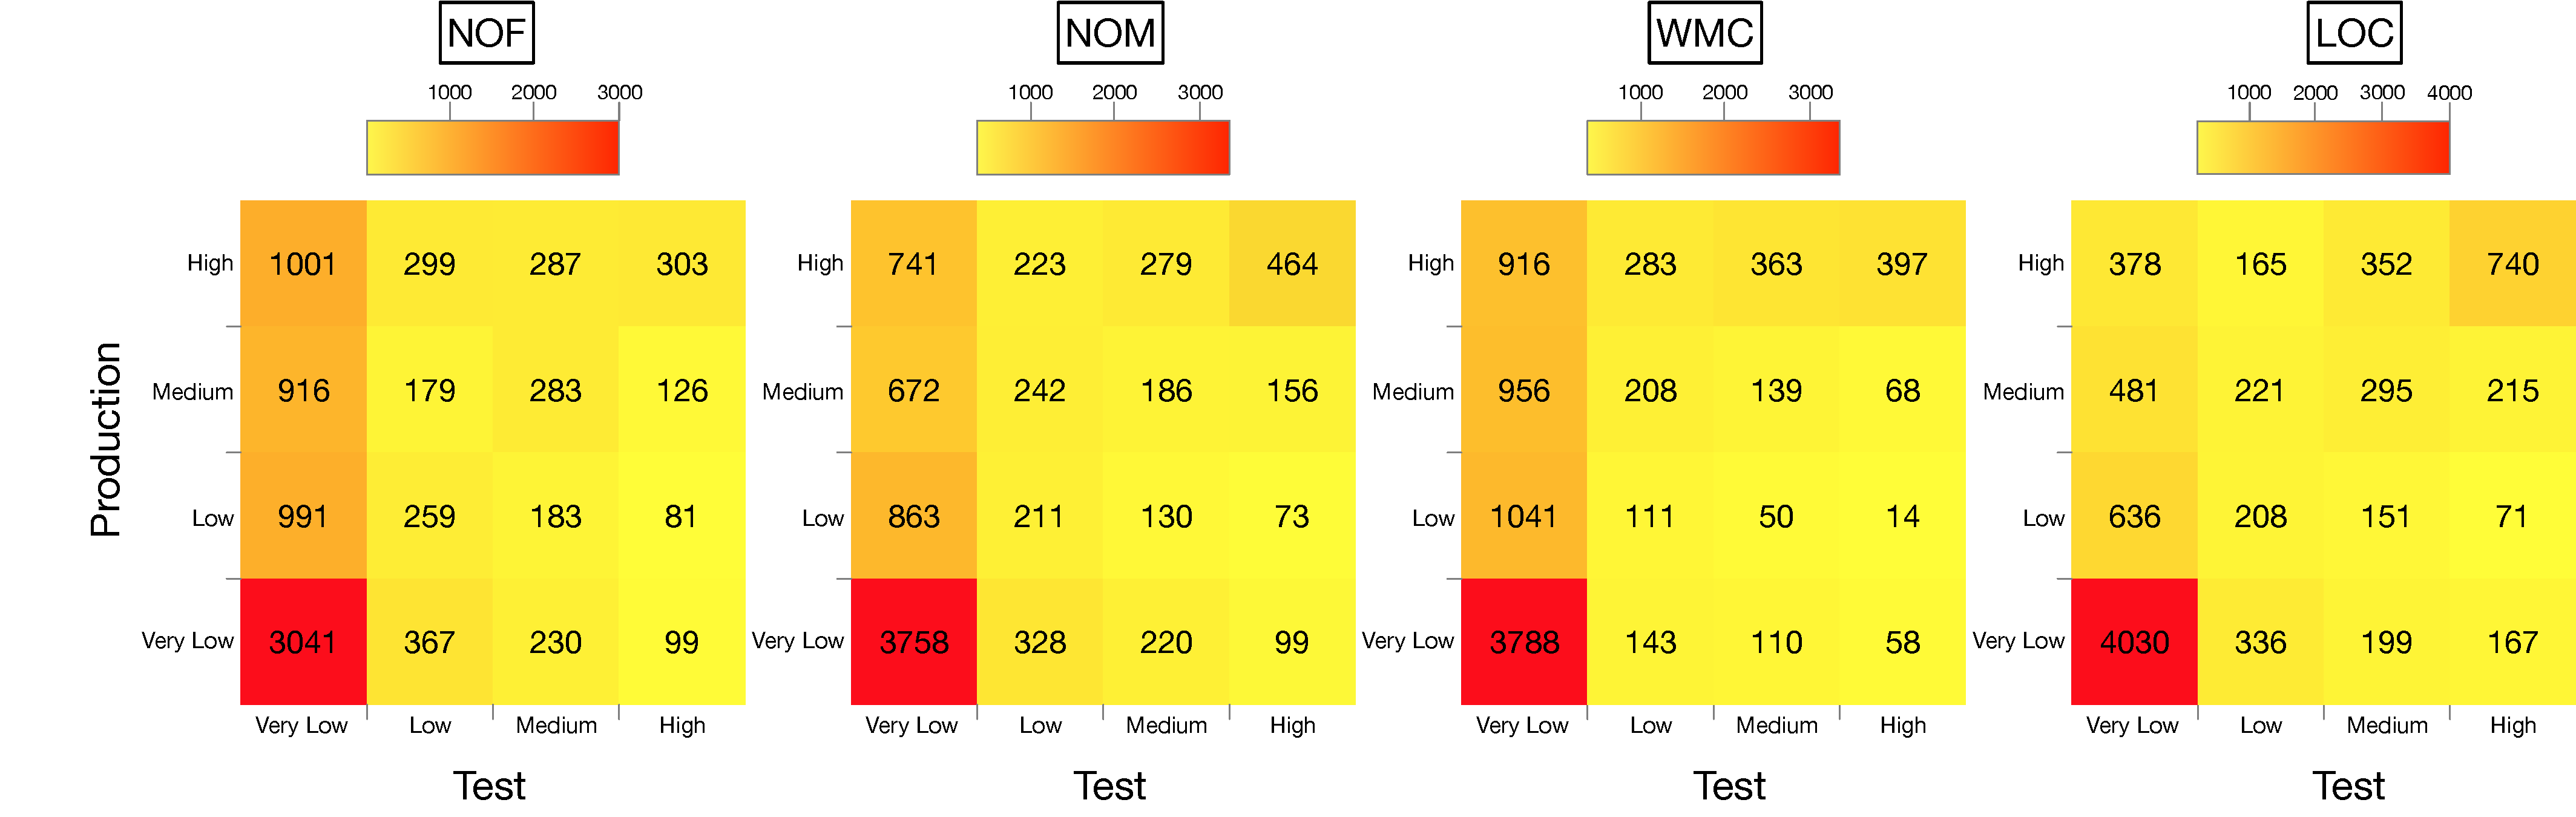
\includegraphics[width=\textwidth]{resources/heat_map.pdf}
    \caption{Categorization of test-production code class pairs for each metric. On the X-axis we find the test categories, while on Y-axis we find the categories of the corresponding production file.}
    \label{fig:heat_map}
\end{figure*}

\section{conclusion}
After analysing the data we have mined and processed we aim to now answer the research questions we have described in section \ref{rqs}.

In section \ref{refactormethods} it was quite obvious that \textit{Rename Method} was by far the most used refactor method from the evaluated repositories, however the refactor methods: \textit{Rename Class} , \textit{Extract Method} and \textit{Move Class} were also used a lot. Despite the fact that these methods were used the most, they were not used consistently over all the repositories. The refactor methods: \textit{Move Attribute}, \textit{Move Method}, \textit{Inline Method} and \textit{Extract Interface} were used around the same amount of times in each project. In order to answer \textbf{RQ1}: \textit{"What type of refactorings do developers apply on testcode?"}, we could say that developers actually use almost all of the evaluated refactor methods on test code, some more than others and not all are consistently used. However, the refactor methods \textit{Extract Interface} and \textit{Rename Package} are barely used at all.

In section \ref{maintainability:improved} we have seen that there were no production classes that somehow had been affected in terms of maintainability after a significant maintainability affecting test refactoring had taken place. With this result we can say that regarding \textbf{RQ2} and \textbf{RQ2.1} the answer to the question \textit{"Does the refactoring of test code affect the maintainability of production code?"} is no, and therefore also it also does not differ per refactoring type.

Finally we have seen in section \ref{maintainability:correlation} that there seems to be a strong correlation in every metric that production classes that are classified as Very Low in terms of risk that their corresponding test class is in this same category. From this we can conclude that there is a correlation however it should be noted that this correlation does not hold for the other categories. We discussed this could be related to the fact that even more complex classes can be tested with relatively simple code, thus resulting in the higher density in the leftmost column in each of the plots shown. Therefore our answer to \textbf{RQ3}: \textit{"What is the correlation between test code maintainability and production code maintainability?"} is that maintainable\footnote{where we say maintainable is being classified as a Very Low risk class} test classes tend to also have maintainable production classes. However is it to be noted that although a large amount of test classes that we have analysed were considered maintainable, their corresponding production classes were classified as less maintainable too\footnote{by this we refer to the higher density leftmost column described in section \ref{maintainability:correlation}}.
\section{Future Work}
A few suggestions for future works, we suggest introducing a more sophisticated refactoring detection tool, we noticed that some commits that include several different refactorings on the same piece of code only got recognized as a single refactoring type, while several were involved. This could give further insights in the results we have found regarding RQ1.

Furthermore we suggest finding a more sophisticated method for asserting software maintainability, perhaps considering several granularity levels, from system to method level. We have seen that there is already several methods proposed, each having their own flaws, we think the CK metrics are a good starting point for the assessment with possibly including the Hallstead complexity measures \cite{halstead1977elements} since they both give insight on the size and complexity of a system or piece of code, which we consider key factors of maintainability.

A further consideration that might prove interesting is to look into the inverse correlation of that we have analysed in RQ2, i.e. is there a correlation between a significant maintainability improving production code refactor and a similar improvement in test code. By analysing this correlation developers might be pushed to keep their test code in as good shape as their production code. Since having higher quality test code has proven to give higher throughput and productivity \cite{athanasiou2011constructing}. 

At last we would recommend using more repositories to evaluate the refactors over the course of a project. During time constraints we were only able to take three repositories into consideration, however since the data has showed us that there is a inconsistency of refactors used over the three projects, we recommend using more repositories to evaluate in order to speculate whether the results are not biased on one specific project.
\section{Acknowledgements}
The authors of this paper gracefully acknowledge the assitance of D. Spadini for giving fast and direct feedback on the research during the course of the project.

\bibliographystyle{abbrv}
\bibliography{bibliography}

\end{document}